\documentclass{tufte-handout}

%\geometry{showframe}% for debugging purposes -- displays the margins



\newcommand{\bra}[1]{\left(#1\right)}
\usepackage{clrscode3e}
\usepackage[activate={true,nocompatibility},final,tracking=true,kerning=true,spacing=true,factor=1100,stretch=10,shrink=10]{microtype}
\usepackage{tikz}
\usepackage{amsmath,amsthm, amssymb}
\usetikzlibrary{shapes}
\usetikzlibrary{positioning}
% Set up the images/graphics package
\usepackage{graphicx}
\setkeys{Gin}{width=\linewidth,totalheight=\textheight,keepaspectratio}
\graphicspath{{.}}

\title{Lecture Notes for COMP 552 - Fall 2018}
\author[Ralph Sarkis]{Ralph Sarkis}
\date{\today}  % if the \date{} command is left out, the current date will be used

% The following package makes prettier tables.  We're all about the bling!
\usepackage{booktabs}

% The units package provides nice, non-stacked fractions and better spacing
% for units.
\usepackage{units}

% The fancyvrb package lets us customize the formatting of verbatim
% environments.  We use a slightly smaller font.
\usepackage{fancyvrb}
\fvset{fontsize=\normalsize}

% Small sections of multiple columns
\usepackage{multicol}

%--------Theorem Environments--------
%theoremstyle{plain} --- default
\newtheorem{thm}{Theorem}
\newtheorem{cor}[thm]{Corollary}
\newtheorem{prop}[thm]{Proposition}
\newtheorem{lem}[thm]{Lemma}
\newtheorem{conj}[thm]{Conjecture}
\newtheorem{quest}[thm]{Question}
\newtheorem{claim}{Claim}

\theoremstyle{definition}
\newtheorem{defn}[thm]{Definition}
\newtheorem{defns}[thm]{Definitions}
\newtheorem{con}[thm]{Construction}
\newtheorem{exmp}[thm]{Example}
\newtheorem{jk}[thm]{Joke}
\newtheorem{exmps}[thm]{Examples}
\newtheorem{notn}[thm]{Notation}
\newtheorem{notns}[thm]{Notations}
\newtheorem{addm}[thm]{Addendum}
\newtheorem{exer}[thm]{Exercise}

\theoremstyle{remark}
\newtheorem{rem}[thm]{Remark}
\newtheorem{ans}[thm]{Answer}
\newtheorem{rems}[thm]{Remarks}
\newtheorem{warn}[thm]{Warning}
\newtheorem{sch}[thm]{Scholium}

\newcommand{\Mod}[1]{\ (\text{mod}\ #1)}
\newcommand{\norm}[1]{\lVert #1 \rVert}
\newcommand{\R}{\mathbb{R}}
\newcommand{\N}{\mathbb{N}}
\newcommand{\Q}{\mathbb{Q}}
\newcommand{\F}{\mathbb{F}}
\newcommand{\Z}{\mathbb{Z}}
\renewcommand{\P}{\mathbb{P}}
\DeclareMathOperator{\Span}{Span}
\DeclareMathOperator{\val}{val}
\DeclareMathOperator{\comp}{comp}
\DeclareMathOperator{\im}{Im}
\DeclareMathOperator{\reg}{Reg}
\DeclareMathOperator{\odd}{\#odd}
\DeclareMathOperator{\dist}{dist}
\DeclareMathOperator{\sbd}{sbd}
\DeclareMathOperator{\capac}{cap}
\DeclareMathOperator{\defic}{def}
\DeclareMathOperator{\rk}{rank}
\DeclareMathOperator{\conv}{conv}
\DeclareMathOperator{\cone}{cone}


% These commands are used to pretty-print LaTeX commands
\newcommand{\doccmd}[1]{\texttt{\textbackslash#1}}% command name -- adds backslash automatically
\newcommand{\docopt}[1]{\ensuremath{\langle}\textrm{\textit{#1}}\ensuremath{\rangle}}% optional command argument
\newcommand{\docarg}[1]{\textrm{\textit{#1}}}% (required) command argument
\newenvironment{docspec}{\begin{quote}\noindent}{\end{quote}}% command specification environment
\newcommand{\docenv}[1]{\textsf{#1}}% environment name
\newcommand{\docpkg}[1]{\texttt{#1}}% package name
\newcommand{\doccls}[1]{\texttt{#1}}% document class name
\newcommand{\docclsopt}[1]{\texttt{#1}}% document class option name

\begin{document}

\maketitle
\begin{abstract}
These are my lecture notes taken during the Combinatorial Optimization class in fall 2018.
\end{abstract}
\tableofcontents
\section{Course Introduction}
This class will be taught by Bruce Alan Reed. The TA is Mashbat Suzuki, his office hours are on Thursday 1:00-5:00pm and on Friday 1:00-3:00pm. There will be optional problem sets given at each lecture and the grading will be 40\% for the midterm and 60\% for the final. More information can be found on the MyCourses page for this course.

Here is a list of problems that are in the scope of this course. More information about these can be found online and in the slides of the first lecture.

\begin{itemize}
	\item Finding the maximum flow in a network.
	\item Finding the minimum cut in a network.
	\item Finding the largest matching in a graph.
	\item The knapsack problem.
\end{itemize}
Some useful terms we will use.
\begin{defn}[Graph coloring]
	Let $G= (V,E)$ be a graph, a \textbf{$k$-coloring} of $G$ is a function $f: V \rightarrow \{1,\dots, k\}$ such that for edges $(u, v) \in E$, $f(u) \neq f(v)$.
\end{defn}
\begin{defn}[Stable set]
	Let $G=(V,E)$ be a graph, a \textbf{stable set} of $G$ is a subset $S \subseteq V$ such that there no vertices in $S$ are adjacent.
\end{defn}
\begin{defn}
	Let $G=(V,E)$ be a graph, a \textbf{clique} in $G$ is a subset $C \subseteq V$ such that all pairs of vertices in $C$ are adjacent.
\end{defn}

Other subjects we are going to cover include linear programming, the ellipsoid method, matroids, submodular functions and multi-commodity flow.

\section{Maximum Matchings}
\subsection{Max-flow Min-cut}
\begin{defn}[Flow network]
	A flow network is a digraph\footnote{A digraph is a graph where edges are ordered pairs of vertices} $G = (V,E)$ with a source and target/sink vertices denoted $s$ and $t$ respectively and a capacity function $c:E\rightarrow \N$.
\end{defn}
The intuition for this object is a network of nodes with a source that generates resources and sends them to a target. The capacity of an edge is the amount of resources that can go through it.
\begin{exmp}
	The road network forms a flow network since each road has a maximum amount of vehicles that can traverse it every hour. The source and target can be two cities, or two neighborhoods.
	The pipeline network for sending oil can also be seen as a flow network.
\end{exmp}
\begin{rem}
	We will assume that there are no parallel edges, no edges entering $s$ and no edges leaving $t$.
\end{rem}
\begin{defn}[$s,t$-cut]
	An $s,t$-cut is a partition $(A,B)$ of the vertices with $s \in A$ and $t \in B$. The capacity of the cut is denoted $\capac(A,B)$ and it is equal to $\sum_{e \in \partial^+(A)} c(e)$.\footnote{We use $\partial^+(S)$ to denote the outgoing edges of a subset $S$ of vertices, $\partial^-(S)$ denotes the incoming edges.}
\end{defn}
\begin{quest}
	Can you design an algorithm that finds the cut with minimum capacity for any graph ? (This is called the min-cut problem)
\end{quest}
\begin{defn}[$s,t$-flow]
	Let $D= (V,E)$ be a digraph and $s\neq t \in V$. A map $f : E \rightarrow \N$ is an $s,t$-flow if it is smaller than the capacity $c$ and $\forall x \in V \setminus\{s,t\}$, the following holds\footnote{We will call this the flow conservation property.}:
	\[ \sum_{e \in \partial^+(x)}f(e) = \sum_{e \in \partial^-(x)}f(e) \]
	We define the value of an $s,t$-flow as follows:
	\[ \val(f) = \sum_{e \in \partial^+(s)}f(e)\]
\end{defn}

\begin{quest}
	Can you design an algorithm that finds the flow with maximum value for any graph ? (This is called the max-flow problem)
\end{quest}
We will answer the two previous questions with the Ford-Fulkerson algorithm. However, we will try to build towards it by starting with a greedy algorithm that attempts to find the max flow. Here is our attempt:
\begin{enumerate}
	\item Set $f(e) = 0$ for all $e \in E$.
	\item Find a path $P$ from $s$ to $t$ such that $f(e) < c(e)$ for any $e \in P$.
	\item Augment the flow along path $P$.
	\item Repeat until you get stuck, namely, you cannot find more paths.
\end{enumerate}
It is not clear why this does not work but we will see an example where the greedy algorithm does not find the max flow.
\begin{marginfigure}
	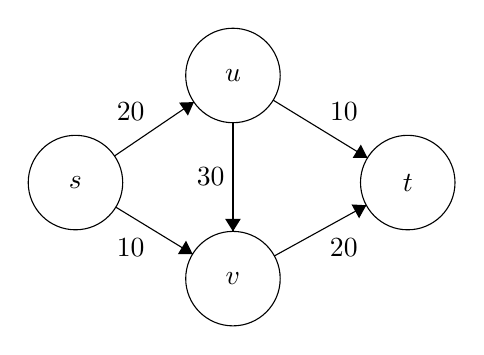
\begin{tikzpicture}[scale=0.2]
	\tikzstyle{every node}+=[inner sep=0pt]
	\draw [black] (16.8,-25.5) circle (3);
	\draw (16.8,-25.5) node {$s$};
	\draw [black] (37.9,-25.5) circle (3);
	\draw (37.9,-25.5) node {$t$};
	\draw [black] (26.8,-18.7) circle (3);
	\draw (26.8,-18.7) node {$u$};
	\draw [black] (26.8,-31.6) circle (3);
	\draw (26.8,-31.6) node {$v$};
	\draw [black] (19.28,-23.81) -- (24.32,-20.39);
	\fill [black] (24.32,-20.39) -- (23.38,-20.42) -- (23.94,-21.25);
	\draw (20.3,-21.6) node [above] {$20$};
	\draw [black] (19.36,-27.06) -- (24.24,-30.04);
	\fill [black] (24.24,-30.04) -- (23.82,-29.19) -- (23.3,-30.05);
	\draw (20.3,-29.05) node [below] {$10$};
	\draw [black] (26.8,-21.7) -- (26.8,-28.6);
	\fill [black] (26.8,-28.6) -- (27.3,-27.8) -- (26.3,-27.8);
	\draw (26.3,-25.15) node [left] {$30$};
	\draw [black] (29.36,-20.27) -- (35.34,-23.93);
	\fill [black] (35.34,-23.93) -- (34.92,-23.09) -- (34.4,-23.94);
	\draw (33.85,-21.6) node [above] {$10$};
	\draw [black] (29.43,-30.16) -- (35.27,-26.94);
	\fill [black] (35.27,-26.94) -- (34.33,-26.89) -- (34.81,-27.77);
	\draw (33.84,-29.05) node [below] {$20$};
	\end{tikzpicture}
	\caption{Flow network for example \ref{greedflow}.}
\end{marginfigure}
\begin{exmp}\label{greedflow}
	On the figure beside, if you start the greedy algorithm with the path $s\rightarrow u\rightarrow v\rightarrow t$ and augment the flow on it by 20, you will end up with the following flow of value 20:
	\begin{center}
		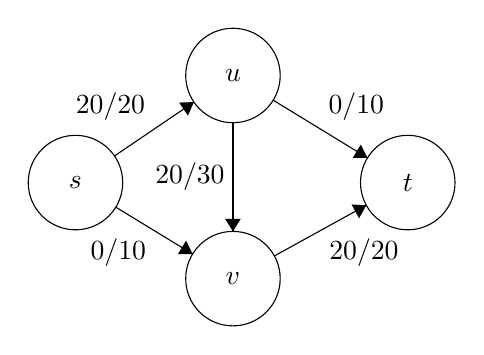
\begin{tikzpicture}[scale=0.2]
		\tikzstyle{every node}+=[inner sep=0pt]
		\draw [black] (16.8,-25.5) circle (3);
		\draw (16.8,-25.5) node {$s$};
		\draw [black] (37.9,-25.5) circle (3);
		\draw (37.9,-25.5) node {$t$};
		\draw [black] (26.8,-18.7) circle (3);
		\draw (26.8,-18.7) node {$u$};
		\draw [black] (26.8,-31.6) circle (3);
		\draw (26.8,-31.6) node {$v$};
		\draw [black] (19.28,-23.81) -- (24.32,-20.39);
		\fill [black] (24.32,-20.39) -- (23.38,-20.42) -- (23.94,-21.25);
		\draw (19.02,-21.6) node [above] {$20/20$};
		\draw [black] (19.36,-27.06) -- (24.24,-30.04);
		\fill [black] (24.24,-30.04) -- (23.82,-29.19) -- (23.3,-30.05);
		\draw (19.52,-29.05) node [below] {$0/10$};
		\draw [black] (26.8,-21.7) -- (26.8,-28.6);
		\fill [black] (26.8,-28.6) -- (27.3,-27.8) -- (26.3,-27.8);
		\draw (26.3,-25.15) node [left] {$20/30$};
		\draw [black] (29.36,-20.27) -- (35.34,-23.93);
		\fill [black] (35.34,-23.93) -- (34.92,-23.09) -- (34.4,-23.94);
		\draw (34.63,-21.6) node [above] {$0/10$};
		\draw [black] (29.43,-30.16) -- (35.27,-26.94);
		\fill [black] (35.27,-26.94) -- (34.33,-26.89) -- (34.81,-27.77);
		\draw (35.12,-29.06) node [below] {$20/20$};
		\end{tikzpicture}
	\end{center}
	Since there is no more valid path, you are stuck, but the max flow has value 30 (try to find it). One can observe that if we started with the path $s\rightarrow v \rightarrow t$, the greedy algorithm would have found the max flow.
\end{exmp}

In order to get to the Ford-Fulkerson algorithm, we need one final key notion.
\begin{marginfigure}
	\begin{center}
		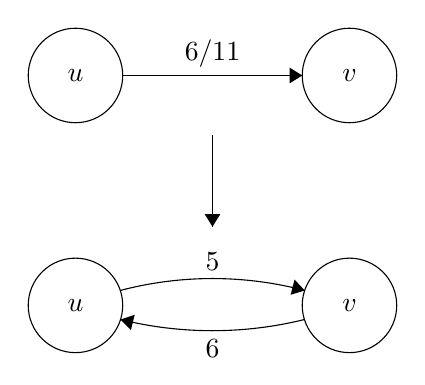
\begin{tikzpicture}[scale=0.2]
		\tikzstyle{every node}+=[inner sep=0pt]
		\draw [black] (16.1,-15.4) circle (3);
		\draw (16.1,-15.4) node {$u$};
		\draw [black] (33.5,-15.4) circle (3);
		\draw (33.5,-15.4) node {$v$};
		\draw [black] (16.1,-30) circle (3);
		\draw (16.1,-30) node {$u$};
		\draw [black] (33.5,-30) circle (3);
		\draw (33.5,-30) node {$v$};
		\draw [black] (19.1,-15.4) -- (30.5,-15.4);
		\fill [black] (30.5,-15.4) -- (29.7,-14.9) -- (29.7,-15.9);
		\draw (24.8,-14.9) node [above] {$6/11$};
		\draw [black] (18.944,-29.051) arc (104.72092:75.27908:23.046);
		\fill [black] (30.66,-29.05) -- (30.01,-28.36) -- (29.76,-29.33);
		\draw (24.8,-27.79) node [above] {$5$};
		\draw [black] (30.639,-30.897) arc (-76.12399:-103.87601:24.348);
		\fill [black] (18.96,-30.9) -- (19.62,-31.57) -- (19.86,-30.6);
		\draw (24.8,-32.11) node [below] {$6$};
		\draw [black] (24.8,-19.2) -- (24.8,-25);
		\fill [black] (24.8,-25) -- (25.3,-24.2) -- (24.3,-24.2);
		\end{tikzpicture}
	\end{center}
	\caption{Example of how an edge gets transformed in residual graph.}
\end{marginfigure}
\begin{defn}[Residual graph]
	Let $(G,s,t,c)$ be a flow network and $f$ an $s,t$-flow, the residual graph is $G_f = (V,E_f)$ where $E_f = \{e \in E \mid f(e) < c(e)\} \cup \{e^{R} \mid f(e) > 0\}$ ($e^{R}$ is the edge $e$ in the reverse direction). It also has the new capacity function $c_f$, that behaves like so: $c_f(e) = c(e) - f(e)$ and $c_f(e^R) = f(e)$.
\end{defn}
\begin{defn}
	An augmenting path of $f$ is a path in $G_f$.
\end{defn}
\begin{defn}
	The bottleneck capacity of an augmenting path $P$ is the minimum capacity of the edges in $P$.
\end{defn}
We first define the $\proc{Augment}$ subroutine that we will use in the algorithm.
\begin{codebox}
	\Procname{$\proc{Augment}(f,c,P)$}
	\li $b \gets$ bottleneck capacity of $P$
	\li \For each edge $e \in P$ \Do
	\li \If $e \in E$ \Then
	\li $f(e) \gets f(e)+b$
	\li \Else
	\li $f(e^R) \gets f(e^R)-b$
	\li \Return f
	\End \End
\end{codebox}

A key property of this subroutine is that the flow returned has value equal to the value of $f$ plus the bottleneck of $P$.

Now, we give the algorithm (look in the margin for the pseudo algorithm):
\marginnote{\begin{codebox}
		\Procname{$\proc{Ford-Fulkerson}(G,s,t,c)$}
		\li \For all $e \in E$, $f(e) \gets 0$.
		\li $G_f \gets $ residual graph of $G$ and $f$.
		\li \While there is an augmenting path $P$ in $G_f$ \Do
		\li $f \gets \proc{Augment}(f,c,P)$
		\li Update $G_f$. \End
		\li \Return $f$.
\end{codebox}}
\begin{enumerate}
	\item Set $f(e) = 0$ for all $e \in E$.
	\item Find an augmenting path in $G_f$.
	\item Augment the flow using the previous subroutine.
	\item Repeat until there are no more augmenting path.
\end{enumerate}

\begin{quest}
	How do you verify the optimality of a flow ?
\end{quest}
One way to do this is to find an upperbound for the value of any flow. That way, if the flow has value equal to the upper bound, then this flow must be optimal. The sum of the capacities of the edges going out of $s$ is an upper bound\footnote{Also, the sum of the capacities of the edges going in $t$.}. This upper bound is not enough for a general graph. We want to find another upper bound.

We start with some important results.
\begin{lem}[Flow-value]
	Let $f$ be any flow and $(A,B)$ be any cut. The net flow across $(A,B)$ is the value of $f$. The net flow is defined like so:
	\[\sum_{e \in \partial^+(A)}f(e) - \sum_{e \in \partial^-(A)}f(e) = \val(f)\]
\end{lem}
\begin{proof}
	Define the following partition of edges.
	\begin{marginfigure}
		\centering
		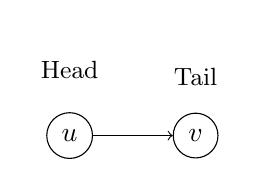
\begin{tikzpicture}[scale=0.8,every node/.style={draw=black,circle}]
		\node[label={\small Head}] (u) at (0,0) {$u$};
		\node[label={\small Tail}] (v) at (2,0) {$v$};
		\draw[->] (u) to (v);
		\end{tikzpicture}
		\caption{Convention for head and tail of edge.}
		\label{fig:orientedge}
	\end{marginfigure}
	\begin{align*}
	E_1 &= \{e \in E \mid \mbox{ head and tail in } A\}\\
	E_2 &= \{e \in E \mid \mbox{ only head in } A\}\\
	E_3 &= \{e \in E \mid \mbox{ only tail in } A\}
	\end{align*}
	We can now expand $\val(f)$:
	\begin{align*}
	\val(f) &= \sum_{e \in \partial^+(s)} f(e)\\
	&= \sum_{e \in \partial^+(s)} f(e) + \sum_{v \in A \setminus \{s\}} \bra{\sum_{e \in \partial^+(v)}f(e) - \sum_{e \in \partial^-(v)}f(e)}\\
	&= \sum_{e \in E_2} f(e) - \sum_{e \in E_3} f(e)
	\end{align*}
\end{proof}

\begin{thm}[Weak duality]
	Let $f$ be any flow and $(A,B)$ be any cut. Then $\val(f) \leq \capac(A,B)$.
\end{thm}
\begin{proof}
	\begin{align*}
	\val(f) &= \sum_{e \in \partial^+(A)}f(e) - \sum_{e \in \partial^-(A)}f(e)\\
	&\leq \sum_{e \in \partial^+(A)}f(e)\\
	&\leq \sum_{e \in \partial^+(A)}c(e)\\
	&= \capac(A,B)
	\end{align*}
\end{proof}
\begin{cor}
	Let $f$ be any flow and let $(A,B)$ be any cut. If $\val(f) = \capac(A,B)$, then $f$ is a max-flow and $(A,B)$ is a min-cut.
\end{cor}
\begin{proof}
	For any flow $f'$, $\val(f') \leq \capac(A,B) = \val(f)$ and for any cut $(A',B')$, $\capac(A',B') \geq \val(f) = \capac(A,B)$.
\end{proof}
With the following two theorems we will show the correctness of the Ford-Fulkerson algorithm (we will show both theorems at the same time).
\begin{thm}[Augmenting path theorem]
	A flow $f$ is a max-flow if and only if no augmenting paths exist in the residual graph $G_f$.	
\end{thm}
\begin{thm}[Max-flow min-cut]
	The value of the max-flow is equal to the capacity of the min-cut.
\end{thm}
\begin{proof}
	We will show the following three conditions are equivalent for any flow $f$.
	\begin{enumerate}
		\item There exists a cut $(A,B)$ such that $\capac(A,B) = \val(f)$.
		\item $f$ is a max-flow.
		\item There is no augmenting path in $G_f$.
	\end{enumerate}
	The equivalence of 1. and 2. is the max-flow min-cut theorem and the equivalence of 2. and 3. is the augmenting path theoreom.
	
	($1 \implies 2$) See previous corollary.
	
	($2 \implies 3$) We prove the contrapositive, if there is still an augmenting path, you can increase the flow so $f$ is not maximum.
	
	($3 \implies 1$) Let $f$ be a flow with no augmenting path in its residual graph. Let $A$ be the set of nodes that are reachable from $s$ in $G_f$ and $B$ be the other nodes, $(A,B)$ defines a cut because there is no augmenting path, implying $t$ is not reachable. We now state two claims. First, every edge $e$ going from $A$ to $B$ must have $f(e) = c(e)$, otherwise, the node in $B$ incident to $e$ would be reachable from $s$. Second, every edge $e$ going from $B$ to $A$ must have $f(e) = 0$, otherwise the node in $B$ would be reachable from $A$ with a backward edge.
	\begin{align*}
	\val(f) &= \sum_{e \in \partial^+(A)}f(e) - \sum_{e \in \partial^-(A)}f(e)\\
	&= \sum_{e \in \partial^+(A)} c(e) &&\mbox{ by the two claims}\\
	&= \capac(A,B)
	\end{align*}
\end{proof}
\begin{rem}
	The cut defined in the proof above is the min-cut. Hence, the Ford-Fulkerson algorithm also gives the min-cut.
\end{rem}
We now look at the runtime of the algorithm. We assume that the capacities are integers between 1 and $C$, $m = |E|$ and $n = |V|$. Observe the integrality invariant: throughout the algorithm, the flow values $f(e)$ and the residual capacities $c_f(e)$ are integers.

\begin{thm}
	The algorithm terminates in at most $\val(f^*) \leq nC$ iterations.
\end{thm}
\begin{proof}
	Every iteration, you increase the value of the flow by at least 1.
\end{proof}
\begin{cor}
	The running time of Ford-Fulkerson is $O(mnC)$.
\end{cor}
\begin{cor}
	If $C = 1$, then running time of Ford-Fulkerson is $O(mn)$.
\end{cor}
\begin{quest}
	Is the generic Ford-Fulkerson algorithm poly-time in input size ($m$, $n$ and $\log(C)$) ?
\end{quest}
Well, if we represent the network as an adjacency matrix where the entries are the capacity, we end up with a representation of size $O(n^2\log C)$ ($\log C$ bits for each of the $n^2$ entries). Hence, the running time $O(mnC)$ is not polynomial time in $C$. There is an example in the slides showing a case where we need more than $O(\log C)$ iterations.

\begin{quest}
	If the weights are not integral, does the algorithm converge to the maximum flow ?
\end{quest}
No.
\subsection{Maximum Cardinality Matching}
Let $G = (A\cup B, E)$ be a bipartite graph. In order to find the max cardinality matching, we use the FF algorithm on the network $G' = (A\cup B \cup \{s,t\}, E \cup \{(s,v) \mid \forall v \in A\} \cup \{(v,t) \mid \forall v \in B\}, s, t, c)$, where  $c(s,v) = 1$ for all $v \in A$ and $c(v,t) = 1$ for all $v \in B$ and $c(e) = \infty$ for any other edge (they are directed from $A$ to $B$).
\begin{prop}
	The max-flow on this network corresponds to the maximum cardinality matching.
\end{prop}
\begin{proof}
	Denote $\val(f^*)$ to be the value of the maximum flow and $\nu(G)$ the maximum cardinality matching of $G$. Since each vertex in $A$ can only receive one unit of flow and each vertex in $B$ can only output one unit of flow, each unit of flow corresponds to a pair of matched vertices. It is then obvious that $\val(f^*) = \nu(G)$.
\end{proof}

Next, we present an algorithm for the general case.

\begin{defn}[Deficiency]
	$\defic(G) = |V(G)| - 2\nu(G)$.\footnote{This corresponds to the number of vertices which are not matched by a maximum matching.}
\end{defn}
\begin{defn}[$M$-exposed]
	Let $G$ be a graph and $M$ a matching of $G$. A vertex of $G$ is called $M$-exposed if no edge of $M$ is incident to $v$.
\end{defn}
\begin{defn}[Alternating and augmenting paths]
	In the same setting, an $M$-alternating path is a path where no two consecutive edges are in the matching and no two consecutive edges are not matched. If, in addition, the endpoints of the path are $M$-exposed, then it is called an $M$-augmenting path.
\end{defn}
\begin{thm}
	$M$ is a maximum matching of $G$ if and only if there are no $M$-augmenting paths in $G$.
\end{thm}
\begin{proof}
	($\Rightarrow$) Suppose $M$ is a maximum matching of $G$ and $P = \{e_1, \dots, e_k\}$ is an $M$-augmenting path, we know that $k$ is odd and $e_j \in M \Leftrightarrow j \text{ is even}$. The symmetric difference $M \ominus P$ has one more edge and we claim it is also a matching of $G$.
	
	Any vertex not in the path is not affected and for every internal vertex of the path, we kept a total of one matching edge incident to it. For the two endpoints, they were not matched by any edge but now they are. Thus, $M \ominus P$ is a matching of $G$.
	
	($\Leftarrow$) Suppose that $M$ is not a maximum matching, then there is a matching $M'$ with one more edge. Let $H = M \cup M'$, it is a collection of paths and cycles since the degree of each vertex cannot exceed 2. Since, there is one more edge in $M'$, there is at least one $M$-augmenting path in $H$ and we are done.
\end{proof}


\begin{thm}[Tutte-Berge formula]
	$$\defic(G) = \max_{X\subseteq V}\bra{\odd(G-X)- |X|}$$
\end{thm}
\begin{lem}
	Let $G$ satisfy the formula and $X_G$ be the maximizer of the R.H.S., then every maximum matching of $G$ matches every vertices of $X_G$.
\end{lem}
\begin{proof}
	Suppose that some matching $M$ of $G$ does not match $u \in X_G$. By definition of $X_G$, there is $\defic(G) + |X_G|$ odd components in $G-X_G$ and each component has at least one vertex that is not matched by $M$ if we remove $X_G$. When we add $|X_G|$, since $u$ is not matched by $M$, we will only be able to match $|X_G|-1$ more vertices in these components. In total, we still have at least $\defic(G) + 1$ un matched vertices which contradicts maximality of $M$.
\end{proof}
\begin{proof}[Proof of Tutte-Berge]
	($\geq$) Let $X$ be a subset of $V$ and $k = \odd(G-X)$. Let $M$ be the maximum matching of $G$. In each odd component of $G-X$, we know one vertex can only be matched with a vertex of $X$. Therefore, $k- |X|$ vertices cannot be matched and $\defic(G) \geq k-|X|$.
	
	($\leq$) Suppose that $G$ is a counter-example with the least number of vertices. It is easy to see that $G$ has at least one edge. For any strictly smaller subgraph $H$, let $X_H$ be a subset of $V(H)$ for which $\odd(H-X_H) = |X_H| + \defic(H)$\footnote{It exists because $G$ is the smallest graph not satisfying the inequality.}. For all such $H$, every vertex of $X_H$ is in every maximum matching of $H$ by the previous lemma.
	
	Suppose there exist $v \in V$ that is in every maximum matching of $G$, then $\defic(G-v) = \defic(G)+1$. Thus, the set $X = v+ X_{G-v}$ shows the formula holds. Hence, no such vertices exist. In particular, there is more than one maximum matching.
	
	For any edge $e = \{u,v\}$, we can find an odd cycle $C$ going through $e$ with $E(V)\setminus \{e\}$ contained in the union of two matchings. Let $M$ and $N$ be maximum matchings such that $v$ is $M$-exposed and $u$ is $N$-exposed\footnote{Note that this implies $M$ matches $u$ and $N$ matches $v$ as otherwise you could add $e$ to the matching.}. In $M\cup N$, we only have paths and cycles and $u$ is the endpoint of one such path $P$. The other endpoint must be matched by $N$, otherwise $P$ would be $N$-augmenting, it is also $M$-exposed because it is the end of the path. If this endpoint is not $v$, then $P \cup \{e\}$ is an $M$-augmenting path, so we get a contradiction.
	If this endpoint is $v$, we are done because $P$ has an even number of edges and $P \cup \{e\}$ is the desired odd cycle $C$.
	
	Let $G*C$ be the graph $G$ after contracting $C$. Namely, the vertices are $V \setminus V(C) \cup\{C\}$ and the edges are $E \setminus \{e \in E \mid |e\cap C| \geq 1\} \cup \{\{v,C\} \mid \exists (v,x) \in E, x \in C, v\notin C\}$.
	
	We can find a matching in $G-V(C)$ that has $\nu(G) - \frac{1}{2}(|V(C)|-1)$ edges\footnote{Pick one vertex of $C$ and a maximum matching where it is exposed. Then, removing all edges in the cycle yields the desired matching.}, so $\nu(G*C) \geq \nu(G) - \frac{1}{2}(|V(C)|-1)$.
	
	Conversely, let $M'$ be a matching in $G*C$, if $C$ is exposed, then we can define a matching $M$ in $G$ by adding $\frac{1}{2}(|V(C)|-1)$ alternating edges of $C$ to $M'$. If $C$ is not exposed, we can still do that by taking an edge in $G$ corresponding to the edge matching $C$ and the same number of alternating edges of $C$ that are not incident to that edge.\footnote{Make a figure with this.} We conclude that $\nu(G*C) = \nu(G) - \frac{1}{2}(|V(C)|-1)$.
	
	Moreover, $C$ cannot be in all maximum matchings of $G*C$ as we have just proved the construction of the matching in $G-V(C)$ (which does not match $C$) is a maximum matching of $G*C$. Thus, $X_{G*C}$ is a subset of $V\setminus V(C)$. The final observation is that $\odd\bra{G-X_{G*C}} = \odd\bra{G*C-X_{G*C}}$, but this holds because $C$ has an odd number of vertices, so the component containing $C$ in $G*C-X_{G*C}$ will stay odd in $G-X_{G*C}$ and vice-versa. We conclude the other inequality from the following.	
	\begin{align*}
		|X_{G*C}|+\odd\bra{G-X_{G*C}} &=|X_{G*C}|+\odd\bra{G*C-X_{G*C}}\\&=\defic(G*C)\\&= |V(G*C)| - 2(\nu(G*C))\\
		&= |V(G)| - |V(C)| + 1 - 2\nu(G) + |V(C)| -1\\
		&= \defic(G)
	\end{align*}	
\end{proof}
We are ready to give an algorithm to find the max matching. The main idea is that at we start with an empty matching and at each iteration, we either increase the size of the matching or show that we have found a maximum matching. Hence, we need a subroutine taking a graph and matching as input and outputting a larger matching or a proof that the matching is the largest. We need some helpful objects for that.

\begin{defn}[Alternating Tree]
	Let $G$ be a graph and $M$ a matching in $G$. A tree rooted at an $M$-exposed node $r$ is called $M$-alternating if every vertex $v$ at odd depth only has one child $c$ such that $\{v,c\}$ is in the matching. We use the notation $A(T)$ for the nodes at odd depth and $B(T)$ for the nodes at even depth. It is clear that $|B(T)| = |A(T)| + 1$. We say that $T$ is maximal if we cannot add vertices and edges to get a bigger alternating tree and if it does not contain an $M$-augmenting path.
\end{defn}

\begin{lem}
	Let $G=(V,E)$ be a graph, $M$ a matching and $T$ a maximal $M$-alternating tree. Suppose that all the edges with an endpoint in $B(T)$ have the other endpoint in $A(T)$. Let $G' = G[V-V(T)]$ and $M' = M \cap E(G')$. The graph $G$ contains an $M$-augmenting path if and only if $G'$ contains an $M'$-augmenting path.
\end{lem}
\begin{proof}
	($\Leftarrow$) If $G'$ has an $M'$-augmenting path, then either it is also an $M$-augmenting path in $G$, or at least one of its endpoints is matched with a vertex in $T$. This vertex must be in $A(T)$, but by definition of an $M$-alternating tree, the vertices matched with $A$ must belong to $B$. We conclude that the latter case is not possible.
	
	($\Rightarrow$) If $G$ has an $M$-augmenting path $P$, then either it is also an $M'$-augmenting path or it contains edges in $T$. Note that there is only one $M$-exposed vertex in $T$, so one endpoint of the path must be outside $T$. Observe that adding the path $P$ yields an alternating tree. Thus, either case where $P$ is a subset of $T$ or not lead to a contradiction of maximality of $T$.
\end{proof}

\begin{defn}[Blossom]
	Let $G$ be a graph and $M$ a matching in $G$. If $P$ is an $M$-alternating path of even length starting at an $M$-exposed vertex and ending in vertex contained in an odd cycle $C$ with $|E(C) \cap M| = \frac{1}{2}(|V(C)|-1)$, then we say $C$ is a blossom and that $P$ is its stem.
\end{defn}
\begin{lem}
	Let $G$ be a graph, $M$ a matching and $C$ a blossom. The graph $G$ contains an $M$-augmenting path if and only if $G*C$ contains one.\footnote{Note that $M$ is clearly a matching in $G*C$ it matches $C$ because $M$ matched one vertex of $C$ with a vertex outside of $C$.}
\end{lem}
\begin{proof}
	($\Leftarrow$)Suppose $G*C$ contains an augmenting path and it is not an $M$-augmenting path in $G$. Then, the path must contain the blossom and without loss of generality, it contains $xCy$, where $xC$ is in $M$. We extend this path to $xa\cdots by$ by adding one half of the cycle of $C$ going from $a$ to $b$, where $a$ is the vertex matched to $x$ and $by$ is the edge corresponding to $Cy$ in $G*C$. The choice of which half is made in order to keep an $M$-alternating path and it is clear that one half will always yield that. This extended path is now an $M$-augmenting path of $G$.
		
	($\Rightarrow$) Suppose $G$ contains an augmenting path, then if we change the matching to $M'$ by swapping the matched and unmatched edges on the stem of $C$, we get a matching of same size as $M$. Thus, $G$ also has an $M'$-augmenting path. If this path does not go through $C$, then it is an $M'$-augmenting path of $G*C$. If it goes through $C$, then stopping this path at $C$ yields an $M'$-augmenting path in $G*C$ because $C$ is $M'$-exposed. Since $|M| = |M'|$ we will also have an $M$-augmenting path.
\end{proof}

The conclusion of this discussion is the main theorem of this section.
\begin{thm}[Blossom Algorithm]
	We can find the maximum matching of a general graph in polynomial time.
\end{thm}
\begin{codebox}
	\Procname{$\proc{MaxMatching}(G=(V,E),M)$}
	\li *****DO THIS*****
\end{codebox}

\begin{lem}
	Let $G= (V,E)$ be a graph. For all $S \subseteq V$, there exists a matching $M$ such that no vertex of $S$ is exposed if and only if there does not exist a set $X \subseteq V$ such that $G-X$ has more than $|X|$ odd components contained in $S$. Furthermore, we can find such an $X$ and $M$ efficiently.
\end{lem}
\begin{proof}
	($\Rightarrow$) If we find $X$ such that $G-X$ has more than $|X|$ odd components contained in $S$, then a matching hitting every vertex of $S$ would need to connect each components to $X$ with at least one vertex which is impossible.
	
	($\Leftarrow$) We construct a graph $G'$ from the original graph $G$. Add a clique $K_{|V|}$ and add edges between every vertices of the clique and the vertices of $G-S$. Since no matching hits all of $S$, there is no perfect matching in $G'$. In particular, $\defic(G') > 0$, thus we can find a set $X'$ such that $\odd(G'-X') > |X'|$. By a parity observation\footnote{For any graph $G$ and $X \subseteq V(G)$, $\odd(G-X) \equiv |X| \Mod{2}$.}, we get $\odd(G'-X') \geq |X'| +2$.
	
	Obviously, $X'$ cannot contain all the vertices in the $K_{|V|}$ clique \footnote{Because there would not be enough vertices left to get $|X'| + 2$ components} and hence, there is one component with every vertex of $G-S-X'$ and $K_{|V|} - X'$ and all the other components are contained in $S$. In total, we get at least $|X'| + 1$ odd components contained in $S$. By letting $X = X' \cap V$, we get the desired set since $|X| \leq |X'|$ and there will be at least as much components in $G-X$.
\end{proof}
\begin{lem}
	When $X$ is maximum. For each odd component $U$ of $G-X$, for all $v \in U$, $G[U] - v$ has a perfect matching.
\end{lem}
\begin{proof}
	Suppose there is no perfect matching and there is no perfect matching, then $G-X$ **COMPLETE**
\end{proof}
\section{An introduction to polyhedral combinatorics}
\subsection{Characterizing closed convex sets}
\begin{defn}[Convex]
	A set $S$ is convex if for every two points $x,y \in S$, and for any $0\leq \lambda \leq 1$, $\lambda x + (1-\lambda)y \in S$.\footnote{It follows by induction that the convex combination of any finite set of points stays in $S$.}
\end{defn}
\begin{exmps}
	\begin{itemize}
		\item[]
		\item In $\R^n$, a hyperplane is the solution to some linear equation $a_1x_1 + \cdots a_nx_n = b$. It also defines two open half-spaces and two closed half-spaces when the equality is replaced by $<$ and $>$ or $\leq$ and $\geq$ respectively.
		
		Suppose a half-space $S$ is defined by $\{x \in R^n\mid \sum_i a_i x_i \vartriangleleft  b\}$\footnote{The symbol $\vartriangleleft$ can be replaced by any of the inequality signs.} and $x, y\in S$. If $\lambda \in [0,1]$, then 
		\begin{align*}
			\sum_i a_i(\lambda x_i + (1-\lambda)y_i) &= \lambda \sum_i a_ix_i + (1-\lambda)\sum_i a_iy_i\\
			&\vartriangleleft \lambda b + (1-\lambda) b = b.
		\end{align*}
		Hence, we conclude that any half-space is convex.
		
		\item Let $I$ be an index set and $\{S_i\}_{i\in I}$ be a family of convex sets. If $x,y \in \cap_I S_i$ and $\lambda \in [0,1]$, then $\lambda x + (1-\lambda)y \in S_i, \forall i \in I$. Thus, $\lambda x + (1-\lambda)y \in \cap_I S_i$ and we conclude that the intersection of convex sets is convex.
		
		\item Let $Ax\leq b$ define the feasible region of an LP. If $x, y$ are in the feasible region, then $A(\lambda x+ (1-\lambda)y) = \lambda Ax + (1-\lambda)Ay \leq \lambda b + (1-\lambda)b = b$. Thus, the feasible region is convex.
	\end{itemize}
\end{exmps}

\begin{defn}[Convex Hull]
	Let $S$ be a finite set of points, the convex hull of $S$ is defined by 
	$$ \conv(S) = \left\{\sum_{i=1}^{n} a_i d_i \mid \sum_{i=1}^n a_i = 1, d_i \in S, n \in \N\right\}.$$
	Equivalently, and including the infinite case, $\conv(S)$ is the intersection of all convex subsets of the ambient space containing $S$ and the smallest convex set containing $S$.\footnote{It follows that the convex hull of any set is convex.}
\end{defn}

\begin{lem}[Separation lemma]
	If $S$ is a closed convex set, then for any $z \notin S$, there exists a closed half-space containing $S$ but not $z$.
\end{lem}
\begin{proof}
	The case of $S = \emptyset$ is trivial. Since $S$ is non-empty and closed, it has a point $y\in S$ that minimizes the distance to $z$.\footnote{Requires an  analysis argument, but this is not the focus here.} Let $c = z-y \neq 0$ and $\delta = \frac{1}{2}(\norm{z}^2 - \norm{y}^2)$, we claim that $c^Tz < \delta$ is a half-space that separates $z$ from $S$.
	
	First we confirm that $z$ is not in the half-space:
	\begin{align*}
		c^Tz &= (z-y)^Tz\\
		&> (z-y)^Tz - \frac{1}{2}(\norm{z-y}^2)\\
		&= z^Tz - y^Tz - \frac{1}{2}(z^Tz - 2y^Tz + y^Ty)\\
		&= \frac{1}{2}(z^Tz - y^Ty)\\
		&= \delta
	\end{align*}
	
	One can also check that $c^Ty < \delta$ with the same method.\footnote{\begin{align*}
			c^Ty &= (z-y)^Ty\\
			&< (z-y)^Ty + \frac{1}{2}(\norm{z-y}^2)\\
			&= z^Ty - y^Ty + \frac{1}{2}(z^Tz - 2y^Tz + y^Ty)\\
			&= \frac{1}{2}(z^Tz - y^Ty)\\
			&= \delta
	\end{align*}}
	Next, suppose toward a contradiction that $x \in S$ and $c^Tx \geq \delta$, then, we get $c^T(x-y) > 0$. Hence, there exists $\lambda \in (0,1]$ such that
	$$\lambda < \frac{2c^T(x-y)}{\norm{x-y}^2}.$$
	Let $w = \lambda x + (1-\lambda)y$, since $S$ is convex, $w \in S$. However, we find that 
	\begin{align*}
		\norm{w-z}^2 &= \norm{\lambda x + (1-\lambda)y - z}^2\\
		&= \norm{\lambda (x-y) + (y-z)}^2\\
		&= \norm{\lambda(x-y) - c}^2\\
		&= \lambda^2\norm{x-y}^2 - 2\lambda c^T(x-y) + \norm{c}^2\\
		&<  2\lambda c^T(x-y) -  2\lambda c^T(x-y) + \norm{c}^2\\
		&= \norm{c}^2
	\end{align*}
	which contradicts the fact that $y$ is the point in $S$ closest to $z$. We conclude $S$ is contained in the half-space.
\end{proof}
\begin{cor}
	A closed set is convex if and only if it is the intersection of a set of half-spaces.
\end{cor}
\begin{proof}
	($\Leftarrow$) We know that half-spaces are convex, so the intersection of a set of half-spaces is convex.
	
	($\Rightarrow$) Let $S$ be convex, then for any point not in $S$, we can use the separation lemma to get a half-space containing $S$ and not that point. The intersection of these half-spaces for every non-member of $S$ can only contain $S$, so it is equal to $S$.
\end{proof}
\subsection{Characterizing bounded polyhedra}
\begin{defn}[Polyhedron]
	A polyhedron is the intersection of a finite set of closed half-spaces.\footnote{It is therefore a closed convex set.} We often define a polyhedron with a matrix $A \in \R^{m\times n}$ and a vector $b\in \R^m$, letting $$P = \{x \in \R^n \mid Ax \leq b\}.$$
\end{defn}
\begin{defn}[Polytope]
	A polytope is the convex hull of a finite set of points.
\end{defn}
\begin{defn}[Vertex]
	A point in a convex set $S$ is a vertex of $S$ if it is not the convex combination of points in $S\setminus\{v\}$.
\end{defn}

Let $P$ be a polyhedron defined by $Ax \leq b$ and $z \in P$, we will denote $A_z$ and $b_z$ to be the submatrices consisting of the rows that are satisfied with equality in $Az \leq b$. In other words, we have $A_zz = b_z$.
\begin{lem}\label{charvertices}
	A point $z$ in a polyhedron given by $Ax \leq b$ is a vertex if and only if there is no $c \neq 0$ such that $A_zc = 0$.
\end{lem}
\begin{proof}
	($\Rightarrow$) We prove the contrapositive. Suppose that there exists a $c \neq 0$ such that $A_zc = 0$. Since for all rows $A_i$ not in $A_z$, $A_iz \neq b_i$, we must have $A_iz < b_i$. Thus, we can find some $\delta > 0$ such that $A_i(z\pm \delta c) < b_i$ for all $A_i$'s not in $A_z$. For the rows of $A_z$, we still get $A_z(z\pm\delta c) = b_z$, so in total, we get two new points $z + \delta c$ and $z - \delta c$ in the polyhedron. Moreover, we can write $z= \frac{1}{2}(z+\delta c) + \frac{1}{2}(z - \delta c)$ implying $z$ is not a vertex.
	
	($\Leftarrow$) We prove the contrapositive. Suppose that $z$ is not a vertex, then it is the convex combination of two points and without loss of generality\footnote{Let $S$ be convex set and $z = \lambda x+ (1-\lambda)y$ for $\lambda \in [0,1]$ and $x,y \in S$. If $\lambda \neq \frac{1}{2}$, we can assume $\lambda < \frac{1}{2}$ (or swap the roles of $x$ and $y$), so $w = x+2\lambda(y-x) = (1-2\lambda)x + 2\lambda y$ is in $S$. Then, $\frac{1}{2}x + \frac{1}{2}w = z$.}, we can write $z = \frac{x+y}{2}$ for $x,y \in S$. Observe that $A_z(x-z) , A_z(y-z) \leq 0$ as $A_zx, A_zy \leq b_z$ and $A_zz = b_z$. However, $y-z = -(x-z)$, so $A_z(y-z) = 0$.
\end{proof}
\begin{lem}
	Polyhedron have finitely many vertices.
\end{lem}
\begin{proof}
	For each submatrix of $A_I$, there is at most one point $z$ of the polytope such that $A_z = A_I$, since otherwise, we would have $A_{z_1}(z_1-z_2) = 0$ implying $z_1$ is not a vertex. Since there are finitely many submatrices, there can only be finitely many vertices.
\end{proof}
\begin{thm}\label{charpolyA}
	Every bounded polyhedron is a polytope.
\end{thm}
\begin{proof}
	We claim that a bounded polyhedron $P$ is the convex hull of its vertices $X = \{x_1, \dots, x_n\}$. Pick $z \in P\setminus X$ such that the number of rows in $A_z$ is maximal, we can find a vector $c$ such that $A_zc = 0$ because $z$ is not a vertex. Since $P$ is closed and bounded, we can find maximal $\lambda_1, \lambda_2 > 0$ such that $z+\lambda_1c$ and $z-\lambda_2c$ are in $P$. Both points satisfy at least one more inequality tightly \footnote{Show this***}, so they are convex combinations of the vertices by maximality of $\text{\#rows}(A_z)$. Since $z$ is convex combination of these points, we conclude that $z \in \conv(X)$.
\end{proof}
\begin{thm}\label{charpolyB}
	Every polytope $P$ is a bounded polyhedron.
\end{thm}
\begin{proof}
	We show this by induction on the dimension of the space $d$. If the polytope is contained in an affine plane, then the result follows by the induction hypothesis. Otherwise, without loss of generality\footnote{By translating $P$.}, we can find some $r>0$ such that $B(0,r)$ is contained in $P$.
	
	Now, define $$P^*= \{y \in \R^d \mid x^Ty \leq 1, \forall x \in P\}.$$
	Note that because each $x$ is a convex combination of the vertices $x_1, \dots, x_n$ of $P$, we can also write $$P^* = \{y \in \R^d\mid x_i^Ty \leq 1, 1 \leq i \leq n\}.$$
	We claim that $P^*$ is bounded. Indeed, for any $y \in P^*$, let $x = r\frac{y}{\norm{y}}$, this point is in $B(0,r)$, so it is in $P$. We get that 
	$$x^Ty \leq 1 \implies r\norm{y} \leq 1 \implies \norm{y} \leq \frac{1}{r}.$$
	
	This means $P^*$ is a bounded polyhedron and by theorem \ref{charpolyA}, it is a polytope and we have $P^* = \conv(y_1, \dots, y_m)$, where the $y_j$'s are the vertices of $P^*$. Now, we claim that 
	$$P = \{x \in \R^d \mid y_j^Tx \leq 1, 1\leq j \leq m\}.$$
	
	The $\subseteq$ inclusion is clear because $y_j^Tx_i = x_i^Ty_j \leq 1$ for any vertex $x_i$ (thus also for any convex combination of the vertices). For $\supseteq$, suppose that $x$ is in the R.H.S. but not in $P$. By the separation lemma, we can find a hyperplane that separates $x$ from $P$. In mathematical terms, we can find $c\in \R^d$ and $\delta \geq 0$ such that $c^Tx \geq \delta$ and $c^Tx' < \delta$ for all $x' \in P$. Since $0$ is an element of $P$, we cannot have $\delta = 0$, then we can rescale $c$ to have $\delta = 1$.
	
	In conclusion, we obtain that $c^Tx' < 1$ for all $x' \in P$, which means $c\in P^*$. Thus, we can write $c = \sum_{j=1}^m \lambda_j y_j$, with $\sum_j \lambda_j = 1$. However, this leads to the following contradiction:
	$$1 < c^Tx = \sum_{j=1}^m \lambda_j y_j^Tx \leq \sum_{j=1}^m \lambda_j = 1.$$
	
	This means that $P$ is a polyhedron and since it is clearly bounded\footnote{It is the convex hull of a finite set of vertices}, we have shown the theorem.
\end{proof}
\subsection{Characterizing unbounded polyhedra}
\begin{lem}\label{charubpolyA}
	Let $P$ be a polyhedron given by $Ax \leq b$ and $X$ be the vertices of $P$. If there is no non-zero $z$ such that $Az = 0$, then $$P = \conv(X) + \{y \mid Ay \leq 0\}.$$
\end{lem}
\begin{proof}
	($\supseteq$) If $x \in \conv(X)$, then $Ax\leq b$. Thus, if $Ay\leq 0$, then $A(x+y) \leq b$ and $x+y \in P$.
	
	($\subseteq$) Let $w \in P$, we induct on $n-\text{\#rows}(A_w)$.\footnote{Recall that $A_w$ is the set of rows that $w$ satisfies with equality in $Aw \leq b$.} If $w$ satisfies all the rows with equality, then since no $z \neq 0$ yields $A_wz = 0$, $w$ is a vertex \footnote{By lemma \ref{charvertices}.} and, we have $w = w+0$ which is in the R.H.S.
	
	Suppose that $A_w$ does not satisfy all the rows, we can assume that there exists $z\neq 0$ such that $A_wz = 0$, otherwise, we get a vertex again. Replacing $z$ by $-z$ if necessary, we get at least one row $A_i$ of $A$ (not in $A_w$) that yields $A_iz > 0$. For such a row, there is a unique $c_i>0$ such that $A_i(w+c_iz) = b_i$. If we let $c = \min{c_i}$\footnote{The minimum is taken over all rows $A_i$ with $A_iz > 0$.}, wet get that $w+cz$ satisfies one more row with equality and all the other rows are still satisfied. By our induction hypothesis, $w+cz$ is in the R.H.S, so we can write $w+cz = x+ y$ where $x \in \conv(X)$ and $Ay \leq 0$.
	
	If $A(-z) \leq 0$, then $A(y-cz) \leq 0$ and $w = x+(y-cz)$ shows that $w$ in the R.H.S. On the other hand, if $A(-z) > 0$, then we can construct $d$ similarly to $c$ but for $-z$, to get $w-dz \in P$ that satisfies one more row. By induction, it is in the R.H.S. and $w$ is a convex combination of $w+cz$ and $w-dz$ both in the R.H.S., which clearly leads to $w$ being in the R.H.S.
\end{proof}
\begin{lem}\label{charubpolyB}
	Let $P$ be a polyhedron given by $Ax\leq b$ and $X$ be the vertices of $P$. If there exists a non-zero $z$ such that $Az = 0$, then 
	$$P = \{x \in \R^d \mid Ax \leq b, z^Tx = d\} + \{\lambda z \mid \lambda \in \R\}.$$
\end{lem}
\begin{proof}
	($\subseteq$) Let $x \in P$, we know that $Ax \leq b$, so if $z^Tx = d$, we are done. Suppose that $z^Tx = d+ c$ for some $c \in \R$. Let $\lambda = \frac{c}{\norm{z}^2}$ and $y=x-\lambda z$, we have $Ay\leq b$ and $z^Ty = d$.\footnote{\begin{align*}
			Ay  = Ax - A\lambda z = Ax\leq b\\
			z^Ty = z^T(x-\lambda z) = d+c - \lambda \norm{c}^2 = d
			\end{align*}}
	Then, we can write $x = x-\lambda z + \lambda z$ which is in the R.H.S.
	
	($\supseteq$) Let $x$ be in the R.H.S., then write $x = y+\lambda z$ with $Ay \leq b$ and $z^Ty = d$. We have $Ax = A(y+\lambda z) = Ax \leq b$, so $x \in P$.
\end{proof}
\begin{thm}
	A polyhedron is the sum of two convex sets.
\end{thm}
\begin{proof}
	Follows trivially from the two previous lemmas.
\end{proof}

\begin{defn}[Cone]
	A set $S$ is a cone if for any $z$ and $y$ in $S$ and $\lambda, \mu\geq 0$, $\lambda z + \mu y$ is in $S$. For a finite set $X$, the set $\cone(X) = \{\sum_{x \in X} \lambda_x x\mid \forall \lambda_x \geq 0\}$ is a cone.\footnote{It is the smallest cone containing $X$.} A cone is finitely generated if it is $\cone(X)$ for some finite set $X$.
\end{defn}
\begin{prop}
	A cone is convex.
\end{prop}
\begin{proof}
	It follows trivially from the definition as convex combinations are of the form $\lambda z + \mu y $ for $\lambda , \mu > 0$.
\end{proof}
\begin{prop}
	For all matrices $A$, $\{y\in \R^d \mid Ay\leq 0\}$ is a finitely generated cone.
\end{prop}
\begin{proof}
	We proceed by induction on $d-\text{rank}(A)$, the result is trivial when $A$ is full rank as $\{Ay \leq 0\}$ is generated by $\{-A_i\mid A_i \text{ is a row of } A\}$.\footnote{Indeed, if we let the rows $A_i$ be the basis of our space, $-A$ becomes the $-Id$ and $-Ay\leq 0$ implies all the coordinates of $y$ in this basis are positive.} If there exists $z\neq 0$ such that $Az = 0$, then using the same method as in lemma \ref{charubpolyB}, we get that our cone is the sum of $\{y\mid Ay \leq 0, z^Ty = 0\}$ and $\{\lambda z \mid \lambda \in \R\}$.
	
	The first term in the sum can be rewritten as 
	$$\{y \mid Ay \leq 0, z^Ty \leq 0, -z^Ty \leq 0\} = \{y\mid A'y\leq 0\},$$
	where $A'$ has a higher rank than $A$.\footnote{Because $z$ was orthogonal to all other rows in $A$.} By our induction hypothesis, it is finitely generated by a set $X$. If we add $z$ and $-z$ it is clear that we can generate $A$, showing that it is finitely generated.
	
	Suppose there is no non-zero $z$ such that $Az = 0$. We will show by induction on $t$ that for any $0 \leq t \leq \text{\#rows}(A)$, there is a finite set $S_t$ contained in the cone that generates every point in the cone satisfying exactly $\text{\#rows}(A) -t$ rows of $A$ with equality. If $t=0$, since $Az = 0$ for no non-zero $z$, the set $S_0 = \{0\}$ works.
	
	When $t> 0$, let $B$ be a submatrix of $A$ with $\text{\#rows}(A) -t$ rows. If some point in the cone satisfies the rows of $B$ with equality, call it $w_B$. We know that $w_B$ does not satisfy all rows of $A$ with equality, so one row of $A_b$ is such that $(A-B)_i(-w_B) > 0$. Then, for any $w$ in the cone satisfying the rows of $B$ with equality, we can find $c_{w,i}$ such that $(A-B)_i(w-c_iw_B)=0$ and let $c_w$ be the minimum (running over $i$) of the $c_{w,i}$'s. Then, $w-c_{w}w_B$ satisfies one more row with equality, so it is generated by $S_{t-1}$ by our induction hypothesis. It follows that $$S_t = S_{t-1} \cup \{w_B \mid B \text{ has \#rows}(A) - t \text{ rows}\}$$ generates every point in the cone that satisfy $\text{\#rows}(A) -t$ rows with equality.
\end{proof}

\begin{thm}
	Every polyhedra is the sum of a polytope and a finitely generated cone.
\end{thm}
\begin{proof}
	\footnote{Do it with course notes by Schrijver.}
\end{proof}


\section{Optimizing over the matching polytope}
\begin{defn}[Incidence vector of matching]
	Let $G$ be a graph with $E= \{e_1, \dots, e_m\}$ be the set of edges and $M \subseteq E$ be a matching. The incidence vector of $M$ is $\chi^M$\footnote{We sometimes subscript this vector with an edge $e \in M$ instead of a number.} where
	$$\chi^M_i = \begin{cases}1 &e_i \in M\\0 & \text{o/w}\end{cases}.$$
\end{defn}

\begin{defn}[Matching Polytope]
	The matching polytope of a graph $G$ is the convex hull of the incidence vectors of all matchings of $G$.\footnote{We denote it $MP(G)$.}
\end{defn}

\begin{prop}
	Let $c \in \R^d$, $b \in d$ and $D \subseteq \R^d$ be finite. If all $v \in D$ satisfy $c^Tv \leq b$, so do all $x \in \conv(D)$.
\end{prop}
\begin{proof}
	Let $x \in D$, we know there exists $\lambda_i$ such that $\sum_i \lambda_i v_i = x$ for $v_i \in D$ and $\sum_i \lambda_i = 1$. Thus, we get 
	$$c^Tx = \sum_i \lambda_i c^Tv_i \leq \sum_i \lambda_i b = b.$$
\end{proof}
\begin{prop}\label{mpgalmost}
	For any graph $G$,\footnote{The notation $\partial(v)$ means all edges incident to $v$. For a subset $X \subseteq V(G)$, $\partial(X)$ means the edges that cross the boundary of $X$, in other words, edges with exactly one endpoint in $X$.} $$MP(G) \subseteq \{x\in \R^d \mid x \geq 0\} \cap \{x \in \R^d \mid \forall v \in V, \sum_{e \in \partial(v)} x_e \leq 1\}.$$
\end{prop}
\begin{proof}
	It is clear that for every matching $M$, $\chi^M \geq 0$, so by the last proposition, it holds for any point in $MP(G)$. Moreover, for each matching $M$, $\sum_{ e\in \partial(v)} \chi^M_e \leq 1$ as the $M$ cannot match the same vertex twice, thus this inequality also holds for all points in $MP(G)$.
\end{proof}
However, this is not the full characterization of $MP(G)$ as the following proposition shows.
\begin{prop}
	For all odd cycles $C$ of $G$ (of size $2k+1$), let $x$ be the vector such that $x_e = \frac{1}{2}$ when $e \in E(C)$ and $x_e = 0$ otherwise. $x \notin MP(G)$.\footnote{Note that $x$ is in the R.H.S. of equality in proposition \ref{mpgalmost} but not in $MP(G)$.}
\end{prop}
\begin{proof}
	For any matching $M$, for any odd cycle $C$, $M$ must miss at least one vertex. Thus, if you sum up the $\chi^M_e$ for each edge $e$ in the cycle, you will always be less than $|V(C)|/2$. Thus, any convex combinations of the matchings cannot achieve that but $x$ does, so $x \notin MP(G)$.
\end{proof}
Note that this can be generalized to any set of odd size, and Edmonds' theorem shows this was precisely what was missing from the characterization of the matching polytope. 

\begin{thm}[Edmonds]\label{edmonds}
	$x$ is a convex combination of incidence vectors of matchings of $G$ if and only if it satisfies the following:
	\begin{enumerate}
		\item For all $e \in E(G)$, $x_e \geq 0$.
		\item For all $v \in V(G)$, $\sum_{e \in\partial(v)} x_e \leq 1$.
		\item For all $S \subseteq V(G)$ with $|S|$ odd, $\sum_{e \in E(S)} x_e \leq \frac{|S|-1}{2}$.
	\end{enumerate}
\end{thm}

We first show the version for the perfect matching polytope.

\begin{defn}
	The perfect matching polytope of a graph $G$ is the convex hull of incidence vectors of perfect matchings of $G$.\footnote{We denote it $PMP(G)$.}
\end{defn}

\begin{thm}\label{edmondsperfect}
	A point $x$ is in $PMP(G)$ if and only if it satisfies the following\footnote{Observe that we have to make the second condition a bit tighter because every vertex must be covered by a perfect matching.
	}:
	\begin{enumerate}
		\item For all $e \in E$, $x_e \geq 0$.
		\item For all $v \in V$, $\sum_{e \in \partial(v)} x_e = 1$.
		\item For all $S \subseteq V$ with $|S|$ odd, $\sum_{e \in E(S)} x_e \leq \frac{|S|-1}{2}$.
	\end{enumerate}
\end{thm}
\begin{proof}
	Let $Q(G)$ be the polytope defined by the conditions above, we want to show that $Q(G) = PMP(G)$. The $\supseteq$ inclusion is trivial because the vertices of $PMP(G)$ all satisfy these conditions. For $\subseteq$, assume it is not true, then let $G$ be the graph with $|V| + |E|$ minimal such that $Q(G) \not\subseteq PMP(G)$. Clearly, $|V|$ is even or both polytopes would be empty\footnote{There are no perfect matchings, so $PMP(G)$ is the convex hull of an empty set. If $y \in Q(G)$, then by 3, $\sum_{e \in E} y_e \leq \frac{|V|-1}{2}$, but \begin{align*}
		2\cdot\sum_{e \in E} y_e&= \sum_{v \in V}\sum_{e \in \partial(v)} y_e\\ &= \sum_{v \in V} 1\\ &= |V|
	\end{align*}
which is a contradiction, so $Q(G) = \emptyset$.} and $G$ has at least one vertex and one edge.
	
	We first note that if $x \in Q(G) \setminus PMP(G)$ with $x_e= 0$ for some $e \in E$, then $x \in Q(G-e)$ because we just remove a 0 in the sums of 2 and 3, but we still cannot have $x \in PMP(G-e)$ because any convex combination of perfect matchings not using $e$ is in $PMP(G)$. We obtain a smaller counter example. If $x_e = 1$, then we remove this edge and its endpoints to get $G'$. To check $x \in Q(G')$, we only need to verify 3, which is true because odd sets in $G'$ are odd sets in $G$ and we only removed terms from the sum. We cannot have $x \in PMP(G')$ because we could just extend the matchings in the combination by adding $e$ and we would get $x \in PMP(G)$. Again, this yields a smaller example. We conclude that for any $x \in Q(G)\setminus PMP(G)$ and $e \in E$, we must have $0<x_e< 1$.
	
	However, we have that $\sum_{e \in \partial(v)} x_e =1$ for any $v$, so $v$ must have degree at least 2. We get $|E| \geq |V|$. If it is an equality, then every vertex has degree 2, $G$ is a collection of cycles and the theorem follows either because $G$ has no odd cycle and is bipartite\footnote{Explain why bipartite case is easy.} or because there is an odd cycle and $Q(G) = PMP(G) = \emptyset$. The case $|E| > |V|$ remains.
	
	Now if $Q(G) \not\subseteq PMP(G)$, we can find a vertex $x \in Q(G)$ that is not in $PMP(G)$. This vertex lives in space of dimension $|E|$, so it must satisfy $|E|$ equations tightly. Since it cannot satisfy any equation in 1 and there is not enough equations to satisfy in 2, there exists some odd set $S$ with $\sum_{e \in E(S)} = \frac{|S|-1}{2}$. Let $G' = G*S$ and $G''= G*(G- S)$ be the contractions of the respective sets where we keep parallel edges. Call the contracted vertices $s'$ and $s''$ respectively. We induce two vectors $x'$ and $x''$ for $G'$ and $G''$ from $x$ by removing the irrelevant edges. We claim that $x' \in Q(G')$ and $x'' \in Q(G'')$.
	
	For $x'$, 1 is trivially satisfied. For 2, we only need to check for $s'$ which satisfies the equality because of how we chose $S$. For 3, note that any odd set not containing $s'$ is in $G$, so we only need to check for those containing $s'$. Then, if we replace $s'$ by the elements of $S$, we get an odd set of $G$ which satisfies the inequality and because the edges in its boundary are the same than those on the boundary of the original set, the latter also satisfies the inequality.
	
	For $x''$, the argument is very similar.
	
	Since $G'$ and $G''$ are smaller than $G$, we get that $x'$ and $x''$ are in the respective perfect matching polytopes. Since $x$ is a vertex of $Q(G)$, it has rational entries and so does $x'$ and $x''$. Thus, for some $k \in \N$, we can write 
	$$x' = \frac{1}{k}\sum_{i=1}^k\chi^{M'_i} \quad \quad x'' = \frac{1}{k}\sum_{i=1}^k\chi^{M''_i},$$
	where $M'_i$ and $M''_i$ are perfect matchings in $G'$ and $G''$.
	
	For each $e \in \partial(S)$, we must have $kx'_e$ matchings $M'_i$ that contain $e$ and $kx''_e$  matchings in $M''_i$ that contain $e$ and $kx_e = kx'_e = kx''_e$. However, the $M'_i$'s and $M''_i$'s can only contain one $e \in \partial(S)$, thus, by rearranging the terms, we can make sure that $M'_i$ and $M''_i$ share exactly one $e \in \partial(S)$.
	
	Set $M_i = M'_i \cup M''_i$, it matches all the vertices in $S$ and $G-S$ and has no repeated match because only one $e \in \partial(S)$ is in $M_i$. Hence, it is a perfect matching of $G$ and it is clear to see that 
	$$x = \frac{1}{k} \sum_{i=1}^k\chi^{M_i}.$$
	This implies $x \in PMP(G)$ and we have a contradiction.
	
\end{proof}

\begin{proof}[Proof for $MP(G)$]
	Denote $R(G)$ to be the polyhedron defined by Edmond's characterization, we want to show that $R(G) \subseteq MP(G)$. We will use the result for $PMP(G)$ to make this proof simpler.
	
	Denote $\tilde{G}$ to be a new graph with two copies of $G$ where each vertex is adjacent to its copy.\footnote{Formally, we have $G' = (V',E')$ a copy of $G$ and $\tilde{G} = (\tilde{V}, \tilde{E})$ with
	$$\tilde{V} = V \cup V' \text{ and }\tilde{E} = E \cup E' \bigcup_{v \in V} \{v,v'\}.$$}

	Let $x \in R(G)$, we denote $\tilde{x}$ to be the vector with $\tilde{x}_e = \tilde{x}_{e'} = x_e$ and $x_{\{v,v'\}} = 1- \sum_{e \in \partial(v)} x_e$. Note that if $\tilde{x} \in PMP(\tilde{G})$, then we can restrict to edges of $G$ to obtain a convex combination of matchings of $G$ that yield $x$. In other words, if we can show that $\tilde{x} \in PMP(\tilde{G})$, then we will have that $x \in MP(G)$ and the proof will be done.
	
	We will show that $\tilde{x} \in Q(\tilde{G}) = PMP(\tilde{G})$. It is clear that all inequalities of type 1 are satisfied. The inequalities of type 2 follow from our construction of $\tilde{x}$. Hence, we only have to verify the inequalities of type 3.
	
	Let $\tilde{U}$ be a set of odd size and decompose it as $\tilde{U} = X \cup Y'$ where $X \subseteq V$ and $Y' \subseteq Y'$. Also denote $X'$ to be the copy of $X$ in $V'$ and $Y$ to be the copy of $Y'$ in $V$. Since $|\tilde{U}|$ is odd, we must have that either $|X \setminus Y|$ or $|Y \setminus X|$ is odd.\footnote{ $|\tilde{U}| = |X|+|Y| = |X\setminus Y| + |Y\setminus X| + 2|X \cap Y|$} Without loss of generality, it is the former and because $x \in R(G)$, we have 
	$$\sum_{e \in E[X\setminus Y]} x_e \leq \frac{|X\setminus Y| -1}{2}.$$
	This yields the bound\footnote{For the first inequality, note that when adding up the edges going out of each vertex of $X\setminus Y$, we are counting twice the edges go to another vertex of $X\setminus Y$.}
	\begin{align*}
		\sum_{e \in \partial(X\setminus Y)} \tilde{x}_e &= \sum_{v \in X\setminus Y}\bra{\sum_{e \in \partial(v)}\tilde{x}_e} -2 \bra{\sum_{e \in E[X \setminus Y]} \tilde{x}_e}\\
		&\geq |X\setminus Y| -2 \frac{|X\setminus Y| -1}{2}\\
		&= 1
	\end{align*}
	However, we also have 
	$$\sum_{e \in \partial(\tilde{U})} \tilde{x}_e \geq \sum_{e \in \partial(X\setminus Y) }\tilde{x}_e \geq 1$$
	because although the L.H.S. misses the edges that go from $X\setminus Y$ to $X \cap Y$, it gets enough back from the same edges going from $X' \cap Y'$ to $X'\setminus Y'$. Note that this is equivalent to
	$$\sum_{e \in E[\tilde{U}]} \tilde{x}_e \leq \frac{|\tilde{U}|-1}{2},$$
	since each vertex $v$ satisfies the inequality of type 2. We conclude that $\tilde{x} \in PMP(G)$.
\end{proof}




\end{document}
